%to have line numbers
%\RequirePackage{lineno}
\documentclass[10pt, letterpaper]{article}      
\usepackage[margin=.1cm,font=small,labelfont=bf]{caption}[2007/03/09]
%\usepackage{endnotes}
%\let\footnote=\endnote
\usepackage{setspace}
\usepackage{longtable}                        
\usepackage{anysize}                          
\usepackage{natbib}                           
%\bibpunct{(}{)}{,}{a}{,}{,}                   
\bibpunct{(}{)}{,}{a}{}{,}                   
\usepackage{amsmath}
\usepackage[% draft,
pdftex]{graphicx} %draft is a way to exclude figures                
\usepackage{epstopdf}
\usepackage{hyperref}                             % For creating hyperlinks in cross references

 
% \usepackage[margins]{trackchanges}

% \note[editor]{The note}
% \annote[editor]{Text to annotate}{The note}
%    \add[editor]{Text to add}
% \remove[editor]{Text to remove}
% \change[editor]{Text to remove}{Text to add}

%TODO make it more standard before submission: \marginsize{2cm}{2cm}{1cm}{1cm}
\marginsize{1cm}{1cm}{.5cm}{.5cm}%{left}{right}{top}{bottom}   
					          % Helps LaTeX put figures where YOU want
 \renewcommand{\topfraction}{1}	                  % 90% of page top can be a float
 \renewcommand{\bottomfraction}{1}	          % 90% of page bottom can be a float
 \renewcommand{\textfraction}{0.0}	          % only 10% of page must to be text

 \usepackage{float}                               %latex will not complain to include float after float

\usepackage[table]{xcolor}                        %for table shading
\definecolor{gray90}{gray}{0.90}
\definecolor{orange}{RGB}{255,128,0}

\renewcommand\arraystretch{.9}                    %for spacing of arrays like tabular

%-------------------- my commands -----------------------------------------
\newenvironment{ig}[1]{
\begin{center}
 %\includegraphics[height=5.0in]{#1} 
 \includegraphics[height=3.3in]{#1} 
\end{center}}

 \newcommand{\cc}[1]{
\hspace{-.13in}$\bullet$\marginpar{\begin{spacing}{.6}\begin{footnotesize}\color{blue}{#1}\end{footnotesize}\end{spacing}}
\hspace{-.13in} }

%-------------------- END my commands -----------------------------------------



%-------------------- extra options -----------------------------------------

%%%%%%%%%%%%%
% footnotes %
%%%%%%%%%%%%%

%\long\def\symbolfootnote[#1]#2{\begingroup% %these can be used to make footnote  nonnumeric asterick, dagger etc
%\def\thefootnote{\fnsymbol{footnote}}\footnote[#1]{#2}\endgroup}	%see: http://help-csli.stanford.edu/tex/latex-footnotes.shtml

%%%%%%%%%%%
% spacing %
%%%%%%%%%%%

% \abovecaptionskip: space above caption
% \belowcaptionskip: space below caption
%\oddsidemargin 0cm
%\evensidemargin 0cm

%%%%%%%%%
% style %
%%%%%%%%%

%\pagestyle{myheadings}         % Option to put page headers
                               % Needed \documentclass[a4paper,twoside]{article}
%\markboth{{\small\it Politics and Life Satisfaction }}
%{{\small\it Adam Okulicz-Kozaryn\footnote{I thank \textbf{TODO}. All mistakes
%are mine.}} }

%\headsep 1.5cm
% \pagestyle{empty}			% no page numbers
% \parindent  15.mm			% indent paragraph by this much
% \parskip     2.mm			% space between paragraphs
% \mathindent 20.mm			% indent math equations by this much

%%%%%%%%%%%%%%%%%%
% extra packages %
%%%%%%%%%%%%%%%%%%

\usepackage{datetime}


\usepackage[latin1]{inputenc}
\usepackage{tikz}
\usetikzlibrary{shapes,arrows,backgrounds}


%\usepackage{color}					% For creating coloured text and background
%\usepackage{float}
\usepackage{subfig}                                     % for combined figures

\renewcommand{\ss}[1]{{\colorbox{blue}{\bf \color{white}{#1}}}}
\newcommand{\ee}[1]{\endnote{\vspace{-.10in}\begin{spacing}{1.0}{\normalsize #1}\end{spacing}\vspace{.20in}}}
\newcommand{\emd}[1]{\ExecuteMetaData[/tmp/tex]{#1}} % grab numbers  from stata

%TODO before submitting comment this out to get 'regular fornt'
\usepackage{sectsty}
\allsectionsfont{\normalfont\sffamily}
\usepackage{sectsty}
\allsectionsfont{\normalfont\sffamily}
\renewcommand\familydefault{\sfdefault}

\usepackage[margins]{trackchanges}
\usepackage{rotating}
\usepackage{catchfilebetweentags}

\usepackage{abstract}
\renewcommand{\abstractname}{}    % clear the title
\renewcommand{\absnamepos}{empty} % originally center

\usepackage{pgfplotstable}
% -------------------- END extra options -----------------------------------------
\date{{}\today  \hspace{.2in}\xxivtime}
\title{  % remember to have Vistula University!!
%  Happiness is Flextime, part 2: the opposite of flextime, unpredictability
%\textbf{out of date--aper done in goog doc :(}
%city unhappiness is universal across the deveoped world--no cant say that bc
%they are not significant
The Urban-Rural Happiness Gradient Across Countries% :\\
% City Unhappiness is Common \\ 
% (Despite What Economists Say) %Claims to the Contrary by
}
\author{
% Adam Okulicz-Kozaryn\thanks{EMAIL: adam.okulicz.kozaryn@gmail.com
%   \hfill I thank XXX.  All mistakes are mine.} \\
% {\small Rutgers - Camden  and Vistula University}
}

\begin{document}

%%\setpagewiselinenumbers
%\modulolinenumbers[1]
%\linenumbers

\bibliographystyle{/home/aok/papers/root/tex/ecta}
\maketitle
\vspace{-.4in}
\begin{center}

\end{center}


\begin{abstract}
\noindent This study shows, for the first time, that city unhappiness is 
common across the world. We use the World Values Survey comulative dataset
1981-2020 from \url{www.worldvaluessurvey.org}. 
In all developed countries, % people are happier in smaller places than in large
% places.
 without exception, we find that city dwellers are not happier than rural
residents. This finding is important because it contradicts a common belief that
emerged recently, arguably for ideological reasons \citep[e.g.,][]{glaeser11,glaeser14,burger20}, claiming that urban areas are happier. The effort to contravene the findings that cities tend to be less happy than smaller areas is arguably due to economics axioms: money is centered in cities (production, productivity, income, and consumption increase with population size), and therefore, cities have greater utility, so they must be happier. Yet, empirical evidence says otherwise. 
\end{abstract}
\vspace{.15in} 
\noindent{\sc % Happiness, Life Satisfaction,  Subjective Wellbeing  (SWB),
              % Cities, Urbaniciy, Urban-Rural, Urban-Rural Gradient, World Vaues Survey (WVS)
}
\vspace{.25in} 

Research by \cite{aok11a} provided evidence of an ``urban-rural gradient'' in many countries, where happiness levels rise from lowest in largest cities to highest in smallest places. The gradient is non-linear---the very largest cities are markedly less happy than all other areas in a country, e.g.: New York City \citep{aok_brfss_city_cize16,senior_ny_sep16_14}, London \citep{ons11,ibt13}, Helsinki \citep{morrison15}, Bucharest \citep{lenzi16D}, and Sydney \citep[cited in][]{morrison11}.
The goal of this paper is to test the gradient across countries using one dataset with uniform set of variables. This study shows, for the first time, that city unhappiness is common across the world.\footnote{Most extant research about the urban-rural happiness gradient is about the United States, Western Europe, recently China, and a handful of other countries. These studies were conducted in single countries, not using a uniform dataset across countries. The three apparent exceptions \citep{aokcities,burger20,easterlin10al} do not actually examine a gradient---they all use binary urban-rural operationalizations and present simple mean differences for each country and aggregate results to group of countries in regressions. The Gallup data used by \citet{burger20} and \citet{easterlin10al} are problematic as elaborated later on in this paper.}
 
The intersection of % Quality of Life (QOL), or
 Subjective Wellbeing (SWB) % \footnote{SWB and QOL overlap, but there are important differences, notably QOL is more of an index/aggregate of domains and more subjective, while SWB is subjective mostly an evaluation of one's life as a whole--for a discussion see \citet{aok-swbLivability18}. For simplicity, we use the terms interchangeably throughout the paper.}
 and Urban Studies is an exciting area of research.
Academics, policymakers, administrators, and people in general, have started to pay more
attention to SWB% quality of life indicators
, and not just to monetary measures such
as GDP or income. % It is now commonly accepted, even among economists 
% \citep{stiglitz09al}, that money does not capture the full dimension of subjective wellbeing, being therefore timely to observe human flourishing and examine determinants of happiness for improving quality of life.
 This occurs at a time when the world is experiencing massive
urbanization, arguably the most dramatic change to  way of life of human species \citep{wirth38,hansonCityJournalautumn15}.  It raises the question, how do cities affect the human condition? Do cities affect subjective wellbeing?

% TODO once RR add:
% For review of urbanicitysee \citet{aokCityBook15}. This study is an extension
% and follow-up on \citet{aokcities}. For review of the literature on urbanicity
% and happiness see \citet{aokCityBook15}.

Modern research on the effect of cities on human wellbeing should be rooted on
the extensive classic urban sociological research \citep{tonnies57,wirth38,simmel03,park15,park84}, 
which advanced our knowledge on the negative effect of cities on humans.
%
Quantitative research on the urban-rural happiness gradient dates back to
\cite{gurin60} and \cite{campbell76etal}, who found a significant negative
effect of urbanicity on humans. Over the past several decades, dozens of studies
have concurred \citep[for a review see][]{aokCityBook15}.

Yet, most research in the area examines the United States, Western Europe, and
recently China and only a handful of other countries. Most studies are conducted
focusing on a single country. Hence, we contribute to the literature by using a
uniform dataset across many countries. In what follows, we investigate the relationship between urbanicity and
happiness across the world.

We begin by defining SWB and the mechanisms likely
to link the size of a place to SWB, then discuss the literature and provide a
critical perspective on economic
theory. We present our model, % documenting how we used the received
                                % literature to control for sources of
                                % individual variation,
%rubia that was like verbatim from brian :)
 discuss results, and conclude by discussing the findings. % that urban dwellers are unhappier across the world, when compared to rural residents. 

   
\section*{Subjective Wellbeing}

Subjective wellbeing is an umbrella term for various subjective measures
of wellbeing, notably positive and negative affects, happiness, and life
satisfaction. Most of the SWB research, including this study, uses the life satisfaction measure, which is a global self evaluation of one's life as a whole. This measure is mostly cognitive and not affective---a respondent evaluates her life as whole globally (professional, personal, family, community, etc). The measure captures everything that is going on in one's life---that's a major advantage of the SWB measure over other social and economic indicators aiming at measuring the human condition, progress, and development. The SWB measure is simply the most comprehensive measure possible dwarfing earlier measures such as income, education, or life expectancy  \citep[for a review see][]{diener09}.
%TODO once RR add \cite{aok_lsPol16}
Following usual practice, for simplicity, we use these terms interchangeably: SWB, happiness, and life satisfaction, but specifically we mostly mean life satisfaction as previously defined.

The SWB measure is also at least adequately reliable and valid and considered
acceptable for public policy making and public administration
\citep{diener09,stiglitz09al}, and used frequently in urban research \citep[e.g.,][]{moeinaddini20,mouratidis19,wang19,anon17-cities-oslo,ma17,wkeziak16,valente16,chen15}.

There are cross-cultural comparability caveats, however, and SWB may not be
adequately comparable across countries \citep{kahneman99,diener09}. This limitation should be kept in mind when comparing results across countries in the present study. More focus should be on within-country differences, and this is what this study is mostly about---the difference between smaller and larger places in terms of SWB
within different countries. We treat each country separately and do not pull the data together. In short, one should focus on within-country differences across urbanicity and exercise caution when comparing effects across countries. 

\section*{Definition, Theory, and Potential Causal Mechanism}

This is an observational study, not an experiment, and we don't test causality,
but it is instructive to discuss the potential causal mechanisms driving unhappiness in the largest places.

It is useful to begin with the theory that defines urbanicity and predicts how it would affect SWB. 
We start with the classic urban sociological theory of urban malaise
 \citep{tonnies57,wirth38,simmel03,park15,park84}: cities produce superficiality,
transitoriness, withdrawal, impersonality, superficiality, deviance,
shallowness, anomie, alienation, and cognitive overload.\footnote{The classics
  argued that poor social ties existed in cities, but refer to later arguments by Fischer and his subcultural theory \citep{fischer95,fischer75,fischer72}.} 
Sociological theory does not specify at which point urban malaise arises, there is clearly no hard
cutoff point, rather, the more urban, the more malaise. There may be a certain
threshold though, at which malaise intensifies as hinted at by
\citet{fischer73}: in the largest cities.
In classical urban sociology, a city is defined by a large population size,  density,
and heterogeneity \citep{wirth38}. It is clearly not a binary distinction,
but a gradient:``we should not expect to find abrupt and discontinuous variation
between urban and rural'' \citep[][p. 2]{wirth38}. Thus, we can conclude that urbanicity has mostly a negative effect on humans, and it is rather a continuum than a binary measure, although a threshold at a population of several hundred thousand where malaise intensifies may exist.

Another indication of continuity in the effect of the size of a place on the human condition
comes from physics. There is a physical city constant of 1.15: if you double the
area's population size, many phenomena (e.g. crime, GDP, income, patents)
increase by 15\%
\citep{blissCL_nov4_14,bettencourt10,bettencourt10b,bettencourt07}.\footnote{For
  example, suppose there's a city with a population of 1 million and a murder
  rate of 10 per 100k; for a city twice as big, with a population of 2 million, the murder rate would be 11.5 per 100k, and so on.} 

We would like to especially highlight that for over 95\% of our evolutionary history\footnote{% Already Simmel observed
   % that old cities had a character of today's small town--for instance see
   % \citet[p. 333]{simmel03}.
Per human species evolutionary history, for instance, see the  Encyclopedia Britannica, \url{http://www.britannica.com/EBchecked/topic/277071/hunting-and-gathering-culture}. 
    % Wikipedia
   % \url{http://en.wikipedia.org/wiki/List_of_largest_cities_throughout_history},
   % and  also see .
   For post-medieval history see \citet{white77}.%  World population percent living in cities larger than 100k
   % is from , table 1. 
 } we have lived outside of cities as hunter-gatherers usually in small bands of 50--80 people \citep{maryanski92}.
 This way of life only started to slowly change in about 10,000 B.C.  with the domestication of animals
 and agriculture. The first large cities (larger than several hundred thousand% again,$>$250k
 ) only emerged after 500 B.C. and there were just a handful of them. 
 It was only after industrialization that large cities started to house a noticeable proportion of the population, and only in the 20th century we saw an urbanization explosion---in 1800 a mere 1.7\% of the world population lived in cities larger than 100k, it slowly increased to 2.3\% in 1850,  it doubled to 5.5\% in 1900,
 and  doubled again to 13\% in 1950 \citep{davis55}.

The larger the place, the more the environment differs from the habitat in which we have evolved: dense and crowded,\footnote{There are striking examples of crowding in the largest cities.  To be sure, the majority of the urban population does not live in such extreme crowding, the trend however is in that direction as cities are becoming larger and less affordable. Furthermore, even without extreme crowding, the usual population density is related to crime \citep{bettencourt10b}. There is also evidence that density relates to negative consequences: interestingly, there is evidence that density impacts pathology more than crowding \citep{levy1974effects}. Yet, it is not only density and crowding, other factors such as social support matter as well \citep{cassel2017health}. Some studies didn't find a negative effect of density or crowding and the results were mixed \citep{collette1976urban}. While it seems to be reasonable to assume that density and crowding are positively related, some studies do not find that to be the case \citep{webb1975meaning,rodgers1982density}. Crowding probably has become more common in recent years as cities are becoming less affordable \citep{misraCL15oct6,floridaCL18apr11,weinbergCL16aug11,solariMISC19apr24,schuetzMISC19may7,kotkin_db_mar20_13}.
 For an usefuk discussion and overview of density, crowding and human behavior see \citet{boots1979population,choldin1978urban}.}
airports, subway or rapid transit, tall buildings in downtown, etc. And while urbanness is a continuum, there is a threshold, likely around several hundred thousands of people, when the built environment changes significantly.
%
 There are at least several significantly different stages of urbanicity on the
 urbanness continuum: wilderness, open country, villages, small towns, large towns, cities, large
 cities, and very large cities. Surely, it is difficult to capture urbanness in
 its entirety---most datasets only allow us to analyze a few stages, including the data used
 here---but the point is that treating urbanness as an urban-rural dichotomy \citep[][]{glaeser11,burger20} is an
 oversimplification without much theory to support it.

The biological/evolutionary perspective can be complemented by recent neurological evidence. Urban living is unhealthy to the human brain \citep{lederbogen11} and urban living contributes to the development of psychosis \citep{abrahamyan20}.
 
\section*{Economics and Happiness} % OR COMBINE WITH NEXT ONE
% \section{the three studies on urban rural happiness gradient across countries}

%  , because biased and
% flawed research is produced.
%
% like one by stiupd wolfers too about income and happiness, that it is ot
%quadratic and just take the log lol

Economists try to argue that cities are happier than smaller places, yet, the
overwhelming evidence points to the contrary
\citep{gurin60,campbell76etal,aok11a,aok_brfss_city_cize16,senior_ny_sep16_14,ons11,ibt13,morrison15,lenzi16D,morrison11,aok20}. 
%

The discipline of economics is largely driven by ``axioms'' (the self-evident truths)
or ``laws.''\footnote{No other social science discipline has axioms, and for a good
reason---they do not exist in the social world, and so they should not appear in
social science. See \citet{feynman81} and \cite{davies18} for elaboration.} 
One axiom is that the more money (income or consumption), the greater the
utility \citep[e.g.,][]{autor10}. Utility, however, cannot be measured, thus, it
is often operationalized as or proxied by  ``happiness'' in the discipline:\footnote{Curiously, some economists who do happiness research are skeptical about it at the same time, and do not consider happiness worthy investigation
  \citep[e.g.,][]{deaton13c,glaeser14B,glaeser14}.}:
\begin{equation}
%  income = consumption % (\pm investments and savings)
money = utility \approx happiness
\end{equation}%

Easterlin (\citeyear{easterlin15B,easterlin10B}) and many others have found that
income is unrelated to happiness in the long run at the country level (the so
called Easterlin Paradox). But the finding directly contradicts the economics
axiom, and accordingly economists try to find evidence to the contrary. \citet{stevenson13}, for example, challenged the Easterlin Paradox by claiming to have conflicting ``evidence.''Except, that they studied something different---they examined a different unit of analysis (data at the household level, or across countries at one point in time) and log transformed the data. 

The effort to contravene the finding that cities tend to be less happy than
smaller areas is also arguably due to the economics axiom: money is centered in cities,\footnote{Production, productivity, income, and consumption increase with population size \citep{glaeser11C,glaeser07,glaeser01,rosenthal02,rosenthal03,rosenthal08}.} and therefore, cities have greater utility, and by extension, they must be happier. 
%
 \citet{glaeser11} analyzes only poor countries for his urbanicity--happiness
 analysis, but argues that the relationship holds in general. He contends that
 the positive relationship is ``driven primarily by poorer countries''---and
 leaves the impression that the overall relationship is positive for all
 countries and simply stronger for poorer countries. Empirical evidence,
 however, is incongruent: for most countries the relationship is negative and it
 is only positive in a few cases, typically in the very poorest
 countries. Concurrently, \citet{burger20} states ``in line with earlier
 research, we found that urban populations are, on average, happier than rural
 populations in that they return higher levels of happiness'' and also builds his case by focusing on exceptional outliers, mostly poor African countries. \citet{glaeser14} studies US counties, but retains only cities and drops from his study all other areas. % In addition, the analysis is saturated with many controls, and by adding state-fixed effects, which correlates with population size which flips the relationship from a negative to a positive correlation with urbanicity.
 In contrast, \citet{aok_brfss_city_cize16} using the very same data finds a negative relationship by examining all areas. 
% These studies have contributed to the notion



\section*{What We Know So Far, The Literature}

Most research on the urbanicity--happiness relationship points to an urban-rural happiness gradient, where happiness raises from its lowest level in largest cities, to the highest level in smallest rural areas
\citep[e.g.,][]{campbell76etal,aok11a, aok_brfss_city_cize16,aok20}. 
%
Yet, most research has been conducted in the US or Western Europe, and there are only three cross-country investigations using a common dataset: \citet{aokcities,easterlin10al} and \citet{burger20}.

\citet{easterlin10al} focuses on the effect of economic growth by urban--rural areas and only a small part of the study is about urban--rural differences in SWB, and their results are similar to \citet{aokcities}, who found that in developed countries people are less happy in cities. All three studies, however, are limited. 
%
First, there is no urban--rural gradient in these studies---they all use binary operationalizations, urban v rural. % (or three categories in the case of \citet{aokcities})
 Urbanness or urbanicity is a degree, not a dichotomy.\footnote{Strikingly, \citet{burger20} argues that there is a uniform way to measure urbanicity, which is a mere 3 categories: 1)
Cities, 2) Towns and semi-dense areas and 3) Rural areas; yet, uses a dichotomy
in their study.} Also, the three studies mostly present simple mean differences for each country and aggregate results to groups of countries in regressions and fail to control for necessary predictors of SWB. 

Most critically, there are multiple problems with the Gallup data used by \citet{easterlin10al} and \citet{burger20}.\footnote{\citet{easterlin10al} acknowledge Gallup's limitations and attempts
to address them. \citet{burger20}, on the other hand, does not.}  First, it is not meant for
research but for commerce---Gallup charges \$30,000 (per year) for data access.\footnote{Gallup charges \$30,000 per year for the use of their happiness data (authors'
email inquiry)---private corporations are making a fortune from tax dollars and students tuition---scholars should resist the corporatization of academia \citep{mills2012corporatization,cox2013corporatization,millsNYT12fa,CatropaNYT20feb8,schmidlinNYT15oct10}, and
the corporatization of happiness research \citep{davies15}.} Second, the urbanicity classification is twice less precise than in the World Values Survey (WVS) used in the present study: 4
v 8 categories. Third, while the WVS uses precise population size with numeric cutoffs,
Gallup uses fuzzy concepts such as ``rural area,'' ``small town or village,'' ``large city.''
Fourth, % (and this compounds with the third problem),
Gallup uses self-reports of urbanicity, which is highly
subjective and problematic in this case---many, if not most people, would likely
classify themselves completely arbitrarily into ``rural area'' v ``village'' and so forth. The WVS uses interviewer's information about the place. Fifth, apparently much of the data are missing---\citet{easterlin10al} notes that in 14 countries ``rural area'' responses were exceptionally low.
% Also, 
 About half of the world population is rural, but \citet{burger20} reports that in their
dataset only about a quarter of respondents report rural residence.
%
This study is the first to analyze the urban--rural happiness gradient across countries using a more suitable and accurate dataset. 

\section*{Data And Model}

We use the World Values Survey comulative file 1981-2020 from \url{www.worldvaluessurvey.org}, which is representative of about 90\% of
the world population,\footnote{While the WVS is conducted in about 100 countries
  that represent about 90\% of the world population, due to missing data for
  the particular variables of interest, the present's study coverage is slightly
smaller, covering about 70 countries (depending on the model and specification).} and as elaborated in the previous section, is much better suited for the study than an inadequate and poorly designed Gallup survey. The variables are listed in table \ref{var_des}. 
Country codes and descriptive statistics are in the Supplementary Online
Material (SOM).  % in this study for the models reported in the body of the paper we use XX countries.

The SWB question reads, ``All things considered, how  satisfied are you with your life as a whole these days? Using this card on which 1 means you are `completely dissatisfied' and 10 means you are `completely satisfied' where would you put your satisfaction with your life as a whole?''

Urbanicity is operationalized with the WVS variable ``\texttt{X049},'' objective and recorded by the interviewer, not the respondent.
There are eight categories ranging from '\texttt{<2k}' to '\texttt{>500k}.' This is an
important advantage, because as elaborated earlier, urbanicity or urbanness is a
continuum, not a binary urban v rural dichotomy. We conduct the analysis using a
set of dummy variables for all eight categories (leaving out the base case) in
the SOM. For simplicity and ease of exposition, however,  we present simplified results in the body of the paper using three categories only.
In other words, this study uses 8 categories of urbanicity, and summarizes the results for ease of presentation with 3 categories. Thus, please refer to the SOM for the results of all categories.

Because in many countries, there are either no observations or few observations
in the first two bottom categories \texttt{-2k} and \texttt{2-5k}, we combined
them together for the analyses in the main body of the paper. These two
categories together proxy a city-free natural environment most closely
resembling the natural human habitat where we have evolved, and it includes:
wilderness, open country, and small villages. The other critical category that
must be measured based on the earlier review of theory is large cities. There is likely to be a threshold at several hundred thousand, hence we use the top category on the WVS variable ``\texttt{X049}'' which is `\texttt{>500k}' as a proxy of large cities. Such places, are the least resembling of the natural human habitat and are
mostly consisting of man--made objects such as asphalt, concrete, glass, etc., and
accordingly are likely to be the least happy. Such classification into 
large cities v natural areas produces third category in between, \texttt{5-500k}.
%
% In other word, we are exploring the urbanness gradient fully in the SOM, and
% only then in the second step, for ease of exposition, but preserving original
% findings and patterns, in the body of the paper we simplify it by looking at two extremes
%  \texttt{-5k} v \texttt{500k-}.
The two cutoffs are driven by theory. It would be a gross oversimplification to use
an ubran-rural dichotomy with one cutoff, for example, '\texttt{<100k}' v '\texttt{>100k}' (or any other value). A place never changes abruptly from rural to urban at some cutoff, it is a continuum, it can be simplified to carefully chosen extreme categories, but one must always start with the continuum.
%
Since this aggregation or simplification into 3 categories is still
somewhat arbitrary, we present our alternative aggregations in the supplementary
online material in addition to the full 8-step urbanness gradient. 

% Again the rationale as per theory above is to explore the gradient, the simplest way to do it is to
% contrast smallest v medium and largest places
% this is the key!!! it is not everything is urban or rural as in
%   easterlin or burger! it is rather very rural, say <2k or say <10k v very big
%   >couple hundred thousand; stuff in the middle is mixed; it is a gradient! we
%   use two as gradient illustrative extremes not cassifying everything in
%   between! again gradient is non-linear it is very largest cities v everything
%   else, that dichotomy make sense too, but neither thsi is what easterlin and
%   burger do
% The rationale, as per theory is to 

% It is a gradient raisng from smallest to greatest as argued in
% \citet{aokcities}, hence presentation must be ordinal with multiple categories,
% we have 8 in appendix and can be summarized as smallest v largest; why smallest
% v largest

% \textbf{this is the key!!! it is not everything is urban or rural as in
%   easterlin or burger! it is rather very rural, say <2k or say <10k v very big
%   >couple hundred thousand; stuff in the middle is mixed; it is a gradient! we
%   use two as gradient illustrative extremes not cassifying everything in
%   between! again gradient is non-linear it is very largest cities v everything
%   else, that dichotomy make sense too, but neither thsi is what easterlin and
%   burger do}

% \footnote{There are models with additional controls in SOM (Supplementray
  % Online Material).}

\input{../out/varDesMOD.tex}
 
In the choice of controls we generally follow \citet{aok20}. Table \ref{var_des} lists the control variables used in the body of the
paper and there are specific controls worth discussing.
%
 Young, single and childless persons and young men with tertiary education are
 relatively more satisfied with urban areas as a place of residence \citep{anon-regional-studies-19}.
Income, class,  and education  not only predict greater
 SWB, but are also confounded and higher in cities.\footnote{Simply comparing
   unadjusted means may result in oversimplified or biased research claiming
   that people are happier in cities (e.g. \citep{burger20})---e.g., there is
   confounding of urbanicity with higher income, education and class---see SOM for tables with and without controls.} 
 %ideallly woiuld like cost iof living but missing duh

One great advantage of city life that is often forgotten is freedom, ``City
 air makes men free (Stadt Luft macht frei),'' \citep[p. 12]{park84}\footnote{It originated in the Middle Ages, and it meant freedom from feudalism: non-feudal islands in a sea of feudalism \citep{harvey12}.} hence we control for freedom. 
% 
Likewise, trust is important, as it predicts SWB, and it is lower in cities
 \citep{milgram70}.
 %when RR add my misanthropolis
%
Health is a key predictor of SWB, and the subjective health measure used here is a reasonable measure of actual health \citep{subramanian09b}.

We use a standard OLS regression with robust standard errors.  We treat the 10-step
happiness variable as continuous. An ordinal happiness variable can be treated as a
continuous variable \citep{carbonell04}.
%
OLS has become the default method in happiness research
\citep{blanchflower11}. Theoretically, while there is still debate about the
cardinality of SWB, there are strong arguments to treat it as a cardinal
variable \citep{ng96,ng97}. 

% \pgfplotstableread{
% N    Ans
% 1   -36
% 2    33
% 3   -52
% 4   -22
% 5    33
% 6    38
% 7    48
% 8  -100
% }\mytable

% \pgfplotstabletranspose[string type , colnames from=N, input colnames to=N]\mytablenew{\mytable}
% \pgfplotstabletypeset[string type]{\mytablenew}


%BUG this corrupts the table!!!
% \pgfplotstableread{/tmp/a.txt}{\a}
% \pgfplotstableread{/tmp/b.txt}{\b}
% \pgfplotstableread{/tmp/c.txt}{\c}

% {\scriptsize
% \pgfplotstabletranspose[string type, unbounded coords=jump]\anew{\a}
% \pgfplotstabletypeset[string type]{\anew}
% }

% {\scriptsize
% \pgfplotstabletranspose[string type , colnames from=country, input colnames to=country]\bnew{\b}
% \pgfplotstabletypeset[string type]{\bnew}
% }

% {\scriptsize
% \pgfplotstabletranspose[string type , colnames from=country, input colnames to=country]\cnew{\c}
% \pgfplotstabletypeset[string type]{\cnew}
% }

\section*{Results}

% While, again, we do concern ourselves with the coninuum, the urban-rural happiness
% gradient, results are in the SOM, here for ease of exposition, we only preent
% the contrast between smallest, medium, and largest places.
%
There is a tradeoff in this study between ease of presentation and
elaboration as there are dozens of countries and presenting elaborated
specifications would result in unwieldy presentation---additional specifications
are in the SOM. Here we just present one model that is our full model. It
includes all necessary and some additional controls (yet, not over-saturated
where too many controls would result in collinearity and  many missing observations)---we use here models with controls listed in table
\ref{var_des}. 
 The model presented here uses 3 urbanicity categories, \texttt{<5k (base)}, \texttt{5k-500k},
 and \texttt{>500k}. Results are set in Table \ref{regression}. We are interested in
 the comparison between \texttt{<5k} v \texttt{>500k} because places larger than several
 hundred thousand according to the theory are the most unnatural environment for humans % (as this data allows)
.

%NOTE MANUALLY DELETED -5 column with zeroes and comas for last col
\begin{spacing}{.9} \begin{table}[H]\centering   \begin{scriptsize} \begin{tabular}{p{.5in}p{.5in}p{.5in}p{.5in}p{.5in}p{.5in}p{.5in}p{.5in}p{.5in}p{.5in}p{.5 in}p{.5in}p{.5 in}}\hline \input{../out/exT3-3-manual.tex} \hline * p$<$0.05, $+$ p$<$0.1; robust std err \end{tabular}\end{scriptsize}\caption{\label{regression}OLS regressions of SWB on place size for each country separately controling for predcictors of SWB listed in table \ref{var_des}.%  including year
% dummies (not shown).
}\end{table} \end{spacing}

%adam: for some reason the pdf generated this table as Table 39 instead of Table 2, I am not sure why, so i changed the label to regression to see if that would work. Just make sure you double check this.

The results in table \ref{regression} % for 24 countires are significant, and vast majority, 19 countires, or
show that in 80\% of countries with significant happiness differences across
urbanicity, people are less happy in cities than in smaller areas. The only exceptions are in the East European Post Soviet countries (ALB, ROU, RUS), and in South-Asian countries (BGD and IND). Notably, these are all poor or developing countries. In all developed countries, people are happier in smaller places than in large places---without exception, we find that city dwellers are not happier than rural residents. 

% Results in table \ref{d1} are remarkable. In most countries large cities are less
% happy than small settlements. Remarkably, 
% and the point is that the only ones that are sig and positive are wiers small
% poor and most miserable countries except india and russia which is a big puzzle
%
The conclusion is that in all developed countries studied here, AUS, CAN, DEU, ESP, ITA,
NLD,\footnote{Results  for NLD are only in SOM.} NZL, SWE, USA,  the largest areas are less happy than smaller areas.\footnote{At least in less elaborate specifications shown in the SOM, but even in the most elaborate specifications, even when the coefficient on larger places is insignificant, it is still negative.}

%\textbf{MAYBE LATER}
% make the biggest SWB gaps by country key focus of paper :) 
The urban-rural gradient is greatest in EGY, VEN,\footnote{Note: result for VEN
  should be interpreted with caution---this is the main difference with table
  exT4-3 in SOM and probably has to do with the fact that there are only 60 obs on the base case category. Other results are
  similar between the two tables.} and VNM where the effect sizes are larger than one, while the effect sizes for most other places are small to moderate, around .3 to .5 (on the 1--10 SWB scale).   
%aDAM: THIS TABLE IS MISSING: {exT4-3}
 %
Yet, as indicated earlier, because of the limited cross-cultural comparability of the SWB measure, when interpreting our results, the focus should be on within--country SWB differences across urbanicity, and not on comparing cross--country effect sizes.
% We call for retraction of these fake papers.

It is worth noting that in the first column (5-500k), the majority of the results are
negative with only 5 countries yielding a positive result: GHA, MDA, PER, RUS,
and ZAF---again, what is remarkable is that none of these countries is a
developed country.


\section*{Conclusion And Discussion}

Classic urban sociological theory,
biological/evolutionary mechanism, and neurological evidence point to lower
levels of human wellbeing in cities.
% 
Throughout most of our evolutionary history, humans have lived in small homogeneous groups with low density. As hunters gatherers, humans lived in small bands of 50 to 80 people, later on in simple horticultural society in groups of 100 to 150 people, and in more advanced society these groups reached five to six thousand people \citep{maryanski92}. Hence, unlike other species %\footnote{Human nature is unlike that of bees: by one estimate we're 90\% chimp and only 10\% bee  \citep{haidt12B}.} 
living in heterogeneous, dense, and large settlements, human have not evolved to
live there. Simply put, city living is unnatural to human species. 
%
It is not city problems, such as crime and poverty, but the city itself and its
core characteristics that result in lower wellbeing
\citep{aok_brfss_city_cize16}.  %exT4-3

In the vast majority of countries, the results show a negative effect, and only
positive in East European Post Soviet ALB, ROU, and RUS, and South-Asian BGD and IND.
East European Post Soviet countries are still quite centralized where power, opportunity, and resources are located in the large cities. %So largest places still do have most of the benefits of the central place as per central place theory
India and Bangladesh are curious outliers \citep[for some discussion see][]{deb2020exploring}.
Also note that in about a third or even half of the countries (depending on the
model), there is no SWB difference across urbanicity. This is also a finding
worth reporting as it runs counter to common pro-urbanism and city triumphalism
\citep[e.g.,][]{glaeser11}.
%
One would think that cities are the best places to live as people flock there in doves.
% could Show graph from UN, and the common narrative is that city is the place to be, and so one would think people are happier there.
Thus, a finding showing no difference for many cases is already surprising.

Even as coefficient estimates are small to moderate, the practical significance
of the results is very strong because of the sheer size of urbanization. 
%
Even a minuscule negative effect of .1 (on a scale 1-10) on a large place v a smaller place for a small country of 10 million people translates into an effect equivalent to making 100 thousand people from the most miserable to the most happy on the SWB scale 1-10. % if everyone lived in smaller v larger place
 % Small or moderate effect sizes translate into large effects because of the sheets size of urbanization in billions of people.
 Globally, for billions of people living in cities, there is a massive amount of
 human misery produced. 

Why are people less happy in large cities in the developed world, yet happier in some
developing countries? There is at least one reason. In many developing countries, life is simply unbearable outside of the city lacking necessities such as shelter, food, water, sanitation, and healthcare. In developed countries, even the smallest places have reasonable access to necessities, and they do not suffer from urban disamenities. %burger will save you in addis
                                %abeba and kill yuo in nyc
% Also, it
% may be so that the grass is always greener on the other side--people idealize
% what is missing or what is rare. 
 
As per Maslow's pyramid of needs \citep{maslow87}, survival and opportunity
come first, and this arguably can explain much of the paradox found in this
paper---despite the city being biologically, neurologically, and socially negative
for humans, cities can be useful for human wellbeing at the early stage of a
country's economic development. 


Last but not least, it is important to underscore an alarming trend in higher
education, which is the corporatization of higher education and research
\citep{mills2012corporatization,cox2013corporatization,millsNYT12fa,CatropaNYT20feb8,schmidlinNYT15oct10}. This
includes happiness research \citep{davies15}. `The `World Happiness Report''
\citep{helliwell20} and its chapter about the urban--rural gap in happiness
\citep{burger20} uses data from a private corporation, Gallup, and the report % , and its presentation (e.g., that new zealand happiness conference)
 is largely an advertisement for Gallup. Gallup then sells the happiness data
 for \$30,000 per year per user \footnote{Authors' inquiry to Gallup to use
   their data.}---arguably this is not meant for research (most researchers
 cannot afford it). This is incongruous with what research is meant to do, which
 is to produce unbiased knowledge for the sake of knowledge. Instead, the
 objective of this corporatization of research is to make money---after all, the sole responsibility of a business is to profit \citep{friedman70}.

\section*{Takeaway for Practice}
Humans are worse off in cities (in terms of happiness), but sometimes what
makes us happy is not the right thing to do \citep{linden11,haybron08,nussbaum05}. Notably,
climate change is more important than human happiness, and cities are the most
environmentally friendly type of settlement \citep{meyer13}. Also, there are
some things that can be done to make cities less miserable---we know what can
make a city a relatively happy place of residence  \citep[see][]{ballas13}.

Perhaps the clearest takeaway for practice is that we suffer from overpopulation
and overconsumption. It could be argued that we only need cities because of
overpopulation and climate change \citep{pachauri14}, and not because of
production, productivity, or consumption premium, of cities. In fact,
consumption is already much higher than needed in the developed world, and we need less consumption
\citep{dittmar14,kasser13,leonard10}. We arguably also need less production and less economic growth \citep{kallis12,kallis11,bergh11}. While cities are the most environmentally friendly way to squeeze human overpopulation %adam:missing proper citation \citep{}(MEYER)
to deal better with climate change, cities directly cause climate change by being centers of production and consumption that drives climate change---it's a vicious cycle.  

Concurrently, we would need cities less if we had fewer people
(e.g. contraception, family planning, and sterilization). It is only when there are fewer people that we can have a meaningful discussion about the right city size as we used to have a couple of decades ago.\footnote{It is astonishing that there is no discussion about this. How could we have gone so wrong to think that the bigger the better and that there is no limit---cities are ballooning---Tokyo has about 40 million people, and there are many cities with 20 million residents; In comparison, the greatest and largest cities of antiquity like Ancient Athens had 140 thousand people while Rome had a population of 450 thousand.} 

% % \begin{spacing}{.9}
% %   \begin{table}[H]\centering \caption{Correlation matrix.} \label{sumSta} \begin{scriptsize} \begin{tabular}{@{}
% %           p{1.2in} rrrrrrrrrrrrr @{}}\hline
% %         \input{/tmp/gssLonnie//tmp/ahb2.tex}\hline
% %          \end{tabular}\end{scriptsize}\end{table}
% % \end{spacing}



% Table XXX shows variable distributions. If a variable has more than
% 10 categories it is classified into bins...

% %\input .... %TODO !!!! have input here histograms

% \section*{Additional Descriptive Statistics}
% \label{app_des_sta}

% %make sure i have [H] or h! ???
% % \begin{table}[H]
% % \caption{}
% % \centering
% % \label{}
% % \begin{scriptsize}
% % \input{/tmp/gssLonnie/../out/reg_c.tex}
% % \end{scriptsize}
% % \end{table}

%\newpage
%\theendnotes
\bibliography{/home/aok/papers/root/tex/ebib.bib,swbCityWorld.bib,/home/aok/papers/root/rr/misanthropy-trustCity/tex/trustCity.bib}

\section*{SOM: ONLINE APPENDIX (THIS WILL NOT BE A PART OF THE PAPER}

\subsection*{Descriptive Statistics}

% Note that for ease of presentation numbers were rounded to full digits.
\begin{spacing}{.9} \begin{table}[H]\centering  \label{d1} \begin{scriptsize} \begin{tabular}{lllll}\hline
                                                                                        \input{/home/aok/papers/swbCityWorld/out/lctryMOD.tex}
                                                                                        \hline
                                                                                        % * p$<$0.05, $+$ p$<$0.1; robust std err
                                                                                      \end{tabular}\end{scriptsize}\caption{Country codes.}\end{table} \end{spacing}
%LATER: can show like means of major vars 
        
Some countries were dropped if data were missing on major categories. If there
were less than
30 obs on both collectively 2 smallest categories or on top category a country
was dropped. % These were the following :\textbf{LATER}

\begin{spacing}{.9} \begin{table}[H]\centering  \label{d1} \begin{scriptsize} \begin{tabular}{llllllllll}\hline \input{/home/aok/papers/swbCityWorld/out/lcountMOD.tex} \hline * p$<$0.05, $+$ p$<$0.1; robust std err \end{tabular}\end{scriptsize}\caption{Counts by 8 urbanicity categories on \texttt{X049}.}\end{table} \end{spacing}


\begin{spacing}{1.4} %TODO MAYBE before submission can make it like 2.0
\rowcolors{1}{white}{gray90}

%MEH
% \section*{descriptive stats}

% like in eb paper maybe also like min and max and everything
% in app but order somehow anyway but yeah can see diff in mean across categories
% from bivariate but still median and sd by cat would be useful!
% %adam: guessing that here's where a descriptive stats table will go?!

\subsection*{Limitations}

We do not use the Gallup dataset. Some may argue that this is a limitation because Gallup covers more countries than the WVS. However, given that the Gallup data cost tens of thousands of dollars, we cannot afford it. In fact, we'd discourage scientists from paying from their tax money to private corporations to do research. Therefore, we actually consider it an advantage not to use the Gallup dataset.

Still, many world countries are missing, and using more waves of WVS data in the future as they
become available would contribute significantly to the literature. 

A limitation is that many countries were not included as a result of not having
many people in the smallest or the largest areas. In addition, cross cultural
comparability is a caveat. Hence, we run separate analysis for each country and
don't pool the data together, but still, it should be kept in mind that
happiness can mean something different in different societies. Similarly, cities
around the world are very different. The breadth of the study is accompanied by
oversimplifcation. Some research in this area claims that urban-rural differentials might be country-specific and not be generalisable at all. %adam: proper citations missing here too, fill below and uncomment
%\citep{} and \citep{} (Rees, Tonon, Mikkelsen, \& Rodriguez de la Vega, 2017).''

Again, we would like to have more gradation at the top of the distribution, but
500 thousand is a reasonable and adequate cutoff to distinguish a large city
from other places. Unfortunately, there are no other data better suited for this
purpose and we do best we can with what's available. The results are
conservative---if we had a cutoff at 750 thousand or 1 million, they'd be
stronger \citep{aokCityBook15}.

The limitation of \texttt{X049} is not only a low top bin for largest cities
(500k+), but also about a thrird of values missing. Future research can focus on
specific countries using other data or WVS data using \texttt{X049CS} variable,
which has country specific sizes of places, which however are not directly or
easily comparable--bins differ across countries and in some cases place is names
``major city'', ``Farm / Mountain / Fishing village,'' etc). 


\subsection*{Cities in Developing Countries}

Cities can be actually useful for human wellbeing at the early stage of a
country's development. The graphs \ref{pyramid} and \ref{ingle} elaborate the
Maslow's pyramid mentioned in the body of the paper. At first, one needs to
focus on necessities such as survival and cities do help, which could explain
why people in developing countries are happier there; Yet, it is remarkable that
in all developed countries studied here, people in cities are less happy.

\begin{figure}[H]
\begin{centering}
%\fbox{
 \includegraphics[height=1.2in]{/home/aok/papers/root/old/2011/eurostat_cities/tex/pyramid.pdf}
%} 
 \caption{Place Pyramid, \citep[p 294]{florida08}.} \label{pyramid}
  \end{centering}
\end{figure}

\begin{figure}[H]
\begin{centering}
%\fbox{
 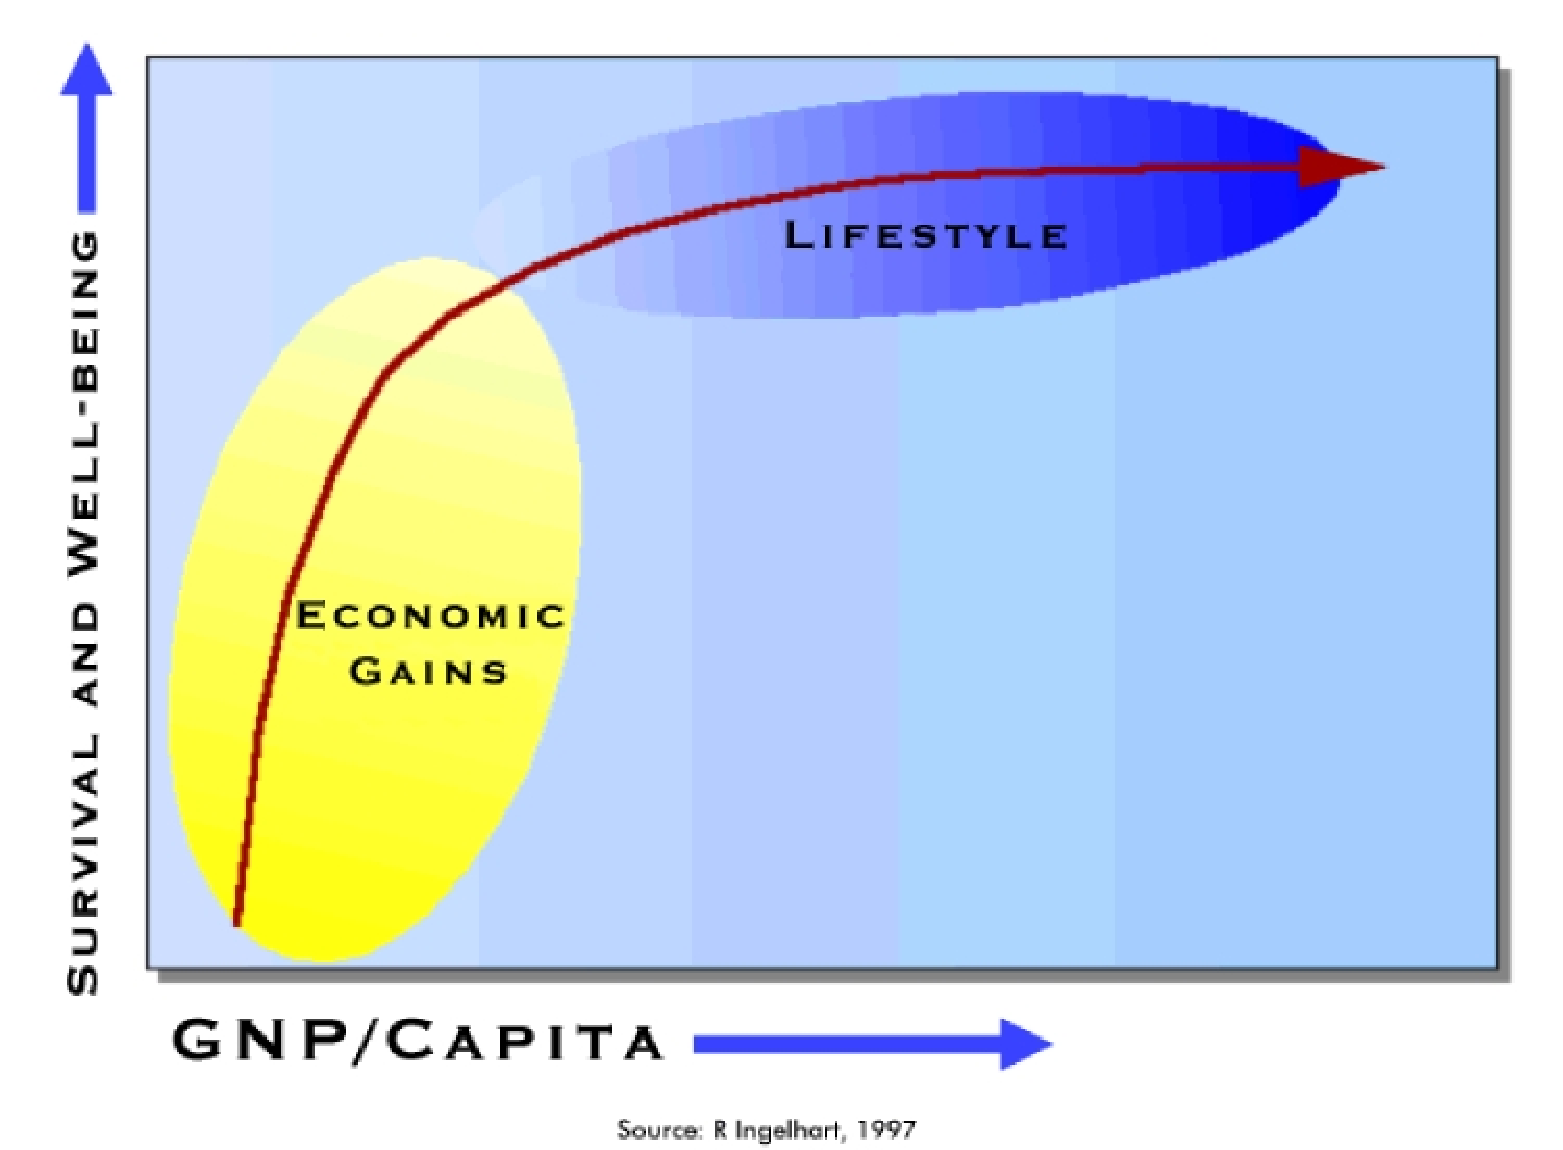
\includegraphics[height=2.5in]{/home/aok/papers/root/old/2011/eurostat_cities/tex/ingle.pdf}
%} 
 \caption{Well-being and income, \citep{inglehart97}.} \label{ingle}
  \end{centering}
\end{figure}


\subsection*{Urbanicity Definition and Operationalization: Alternative Models} 

%adam: the "collapse one way and collapse the other way" below is very unclear, be specific with the cut off points less than 500k and more than 500k
We have three different operationalizations of urbanicity: the original 8
categories, and categories collapsed in 2 alternative ways. There are 4 sets of
models: bivariate (with year dummies), essentially the mean difference between
categories; 2) basic set of controls, necessary/important ones; 3)
full/extended (the one reported in the body); and 4)  over-saturated models,
with many observations missing. 

The models are presented in tables below, where the coding is as follows:
T\# is the type of setup: T is the original 8 categories on the urbanicity
variable; T3 is three categories, and T4 is four categories. 
The number after the dash (-\#) denotes the elaboration of the model:
-1 only includes the urbanicity variable and year dummies\\
-2 adds  age, gender, marital status,  education, income, social class, and health\\
-3 adds materialism, religiosity, automomy, freedom and trust\\
-4 adds crime and financial satisfaction


\begin{spacing}{.9} \begin{table}[H]\centering  \label{exT4-1} \begin{scriptsize} \begin{tabular}{p{1.8in}p{.5in}p{.5in}p{.5in}p{.5in}p{.5in}p{.5in}p{.5in}p{.5in}p{.5in}p{.5 in}p{.5in}p{.5 in}}\hline \input{../out/exT4-1.tex} \hline   * p$<$0.05, $+$ p$<$0.1; robust std err \end{tabular}\end{scriptsize}\caption{exT4-1}\end{table} \end{spacing}

\begin{spacing}{.9} \begin{table}[H]\centering  \label{exT3-1} \begin{scriptsize} \begin{tabular}{p{1.8in}p{.5in}p{.5in}p{.5in}p{.5in}p{.5in}p{.5in}p{.5in}p{.5in}p{.5in}p{.5 in}p{.5in}p{.5 in}}\hline \input{../out/exT3-1.tex} \hline   * p$<$0.05, $+$ p$<$0.1; robust std err \end{tabular}\end{scriptsize}\caption{exT3-1}\end{table} \end{spacing}

\begin{spacing}{.9} \begin{table}[H]\centering  \label{exT-1} \begin{scriptsize} \begin{tabular}{p{1.8in}p{.5in}p{.5in}p{.5in}p{.5in}p{.5in}p{.5in}p{.5in}p{.5in}p{.5in}p{.5 in}p{.5in}p{.5 in}}\hline \input{../out/exT-1.tex} \hline   * p$<$0.05, $+$ p$<$0.1; robust std err \end{tabular}\end{scriptsize}\caption{exT-1}\end{table} \end{spacing}


\begin{spacing}{.9} \begin{table}[H]\centering  \label{exT4-2} \begin{scriptsize} \begin{tabular}{p{1.8in}p{.5in}p{.5in}p{.5in}p{.5in}p{.5in}p{.5in}p{.5in}p{.5in}p{.5in}p{.5 in}p{.5in}p{.5 in}}\hline \input{../out/exT4-2.tex} \hline * p$<$0.05, $+$ p$<$0.1; robust std err \end{tabular}\end{scriptsize}\caption{exT4-2}\end{table} \end{spacing}

\begin{spacing}{.9} \begin{table}[H]\centering  \label{exT3-2} \begin{scriptsize} \begin{tabular}{p{1.8in}p{.5in}p{.5in}p{.5in}p{.5in}p{.5in}p{.5in}p{.5in}p{.5in}p{.5in}p{.5 in}p{.5in}p{.5 in}}\hline \input{../out/exT3-2.tex} \hline   * p$<$0.05, $+$ p$<$0.1; robust std err \end{tabular}\end{scriptsize}\caption{exT3-2}\end{table} \end{spacing}

\begin{spacing}{.9} \begin{table}[H]\centering  \label{exT-2} \begin{scriptsize} \begin{tabular}{p{1.8in}p{.5in}p{.5in}p{.5in}p{.5in}p{.5in}p{.5in}p{.5in}p{.5in}p{.5in}p{.5 in}p{.5in}p{.5 in}}\hline \input{../out/exT-2.tex} \hline   * p$<$0.05, $+$ p$<$0.1; robust std err \end{tabular}\end{scriptsize}\caption{exT-2}\end{table} \end{spacing}


\begin{spacing}{.9} \begin{table}[H]\centering  \label{exT4-3} \begin{scriptsize} \begin{tabular}{p{1.8in}p{.5in}p{.5in}p{.5in}p{.5in}p{.5in}p{.5in}p{.5in}p{.5in}p{.5in}p{.5 in}p{.5in}p{.5 in}}\hline \input{../out/exT4-3.tex} \hline   * p$<$0.05, $+$ p$<$0.1; robust std err \end{tabular}\end{scriptsize}\caption{exT4-3}\end{table} \end{spacing}

\begin{spacing}{.9} \begin{table}[H]\centering  \label{exT3-3} \begin{scriptsize} \begin{tabular}{p{1.8in}p{.5in}p{.5in}p{.5in}p{.5in}p{.5in}p{.5in}p{.5in}p{.5in}p{.5in}p{.5 in}p{.5in}p{.5 in}}\hline \input{../out/exT3-3.tex} \hline   * p$<$0.05, $+$ p$<$0.1; robust std err \end{tabular}\end{scriptsize}\caption{exT3-3}\end{table} \end{spacing}

\begin{spacing}{.9} \begin{table}[H]\centering  \label{exT-3} \begin{scriptsize} \begin{tabular}{p{1.8in}p{.5in}p{.5in}p{.5in}p{.5in}p{.5in}p{.5in}p{.5in}p{.5in}p{.5in}p{.5 in}p{.5in}p{.5 in}}\hline \input{../out/exT-3.tex} \hline   * p$<$0.05, $+$ p$<$0.1; robust std err \end{tabular}\end{scriptsize}\caption{exT-3}\end{table} \end{spacing}





%MEH LATER
% \textbf{So i think start with exT4-2 clean and easy and simple; then exT-3 to
%   show detail and robustness}

% \textbf{TODO meh yeah i guess drop this first table!!!}
% note that all developed countres are less happy in cities, AUS (insiginifacnt
% but sig in next table (\textbf{todo}check!)


In table \ref{exT4-2} several places appear happier like BGD, IND, LTU, PAK, ROU, and RUS, when adding more controls and full town categories that disappear except for 4 countries.


The results in table \ref{exT-3} are remarkable. In most countries, large cities are less happy than small settlements. Without exception, in no developed country the city is a happier place than the smallest areas. The only four countries where people are happier in large cities are: 

% \begin{spacing}{.9}
%   \begin{table}[H]\centering  \label{exT-3} \begin{scriptsize} \begin{tabular}{p{1.8in}p{.5in}p{.5in}p{.5in}p{.5in}p{.5in}p{.5in}p{.5in}p{.5in}p{.5in}p{.5
%             in}p{.5in}p{.5 in}}\hline
%         \input{../out/exT-3.tex}
% \hline  *** p$<$0.001, ** p$<$0.01, * p$<$0.05, $+$ p$<$0.1; robust std err
%          \end{tabular}\end{scriptsize}\caption{exT-3}\end{table}
% \end{spacing}

% The most elaborate model\#4 (-4) has satfin and crime
% like about \textbf{todo count lol} 20/70 neg of all and nly 4/18 of sig are pos
% about 80 perc are neg :) or 5/21 in exT4-3

% and the point is that the only ones that are sig and positive are wiers small
% poor and most miserable countries except india which is a big puzzle

% \textbf{TODO repreat it multiple times!} \textbf{TODO add NOR NLD}
% so the conclusion is that in all develped countries AUS, CAN, DEU, ESP, ITA,
% NZL, SWE, USA,  cities are less happy \footnote{at least in less elaborate
%   specs, but even in most elaborate even if insig, still neg} in vast majority
% of countries effect in ngeative, only positive in these 4:
% russia, moldova and albania are all post soviet countries, they are likely to
% still be very centralized where  power opportunity and resources are located in
% large cities; india is clearly an outlier here and we dont have a good
% explanation \texttt{[blind for peer review]} %\textbf{cite chourjua paper}



% LATER
% show distributuion of place size by country!

% \subsubsection{original 8 categories}
% \subsubsection{0-5k v 500k+}
%yeah this is following berry, but better have 0-5 so that more obs lol

% \subsection{Crime and Cost of Living/financial satisfaction}
% missing obs but here as a robustness check

% TO WHERE I HAVE WE NEED TO CONTROL FOR CRIME:
% Urban unhappiness is not only due
% to urban problems such as crime and poverty.  Cities themselves, their core
% defining characteristics, size and density, are related to unhappiness
% \citep{aok_brfss_city_cize16}. 


% yeh so one limitation is lack of crime; so bias on results cities wiuld be happier otherwhise



\begin{spacing}{.9} \begin{table}[H]\centering  \label{exT4-4} \begin{scriptsize} \begin{tabular}{p{1.8in}p{.5in}p{.5in}p{.5in}p{.5in}p{.5in}p{.5in}p{.5in}p{.5in}p{.5in}p{.5 in}p{.5in}p{.5 in}}\hline \input{../out/exT4-4.tex} \hline   * p$<$0.05, $+$ p$<$0.1; robust std err \end{tabular}\end{scriptsize}\caption{exT4-4}\end{table} \end{spacing}

\begin{spacing}{.9} \begin{table}[H]\centering  \label{exT3-4} \begin{scriptsize} \begin{tabular}{p{1.8in}p{.5in}p{.5in}p{.5in}p{.5in}p{.5in}p{.5in}p{.5in}p{.5in}p{.5in}p{.5 in}p{.5in}p{.5 in}}\hline \input{../out/exT3-4.tex} \hline   * p$<$0.05, $+$ p$<$0.1; robust std err \end{tabular}\end{scriptsize}\caption{exT3-4}\end{table} \end{spacing}

\begin{spacing}{.9} \begin{table}[H]\centering  \label{exT-4} \begin{scriptsize} \begin{tabular}{p{1.8in}p{.5in}p{.5in}p{.5in}p{.5in}p{.5in}p{.5in}p{.5in}p{.5in}p{.5in}p{.5 in}p{.5in}p{.5 in}}\hline \input{../out/exT-4.tex} \hline   * p$<$0.05, $+$ p$<$0.1; robust std err \end{tabular}\end{scriptsize}\caption{exT-4}\end{table} \end{spacing}

% \section{!!!PLAYING DROP THIS LATER}

% \begin{spacing}{.9} \begin{table}[H]\centering  \label{} \begin{scriptsize} \begin{tabular}{p{1.8in}p{.5in}p{.5in}p{.5in}p{.5in}p{.5in}p{.5in}p{.5in}p{.5in}p{.5in}p{.5 in}p{.5in}p{.5 in}}\hline \input{../out/ex1.tex} \hline   * p$<$0.05, $+$ p$<$0.1; robust std err \end{tabular}\end{scriptsize}\caption{ex1}\end{table} \end{spacing}

% \begin{spacing}{.9} \begin{table}[H]\centering  \label{d1} \begin{scriptsize} \begin{tabular}{p{1.8in}p{.5in}p{.5in}p{.5in}p{.5in}p{.5in}p{.5in}p{.5in}p{.5in}p{.5in}p{.5 in}p{.5in}p{.5 in}}\hline \input{../out/ex2.tex} \hline   * p$<$0.05, $+$ p$<$0.1; robust std err \end{tabular}\end{scriptsize}\caption{ex1}\end{table} \end{spacing}



% \subsection{very first results}

% Table \ref{a0} shows resuls of regression of \texttt{SWB} on place size dummies
% (controlling for year dummies), which essentially differences in means for each
% size category. Results are mixed, but large cities (500k-) and even medium sized
% (100-500k) are often happier than the smallest category (the base case or
% reference category, -2k). Usually diferences are small to moderate, about .5 (on
% 1-10 SWB scale), but sometimes large, larger than 1. Do mention the extremes and
% think about why--but we do not have explanation for those. 

% This is what the literature reports, tht results are mixed, in some cases cities
% are happier, in some cases they are not. A key finding of this study is that
% once we properly control for key predictors of SWB, almost uniformly large
% cities (500k-) are less happy than the smallest settlements (-2k). Results are
% shown in the body in table \ref{d1}.


%yah cannot use these 2--didnt drop properly these tiny categories so results
%dont make sense

% \begin{spacing}{.9}
%   \begin{table}[H]\centering \caption{.} \label{d1} \begin{scriptsize} \begin{tabular}{p{1.8in}p{.5in}p{.5in}p{.5in}p{.5in}p{.5in}p{.5in}p{.5in}p{.5in}p{.5in}p{.5
%             in}p{.5in}p{.5 in}}\hline
%         \input{/tmp/a0.tex}
% \hline  *** p$<$0.001, ** p$<$0.01, * p$<$0.05, $+$ p$<$0.1; robust std err
%          \end{tabular}\end{scriptsize}\caption{a0 OLS regressions of
%          \texttt{swb} on \texttt{place size}, controls (not shown) are: enumerate}\end{table}
% \end{spacing}

% Results in table \ref{a} are remarkable. In most countries large cities are less
% happy than small settlements. Remarkably, in no developed country city is
% happier than smallest areas (with exception of KWT and SAU--these are
% middle eastern and oil rich, where cities are glorious indeed)--and they are not
% developed countries according to IMF or UN anyway neither have very high HDI.

% \begin{spacing}{.9}
%   \begin{table}[H]\centering \caption{.} \label{d1} \begin{scriptsize} \begin{tabular}{p{1.8in}p{.5in}p{.5in}p{.5in}p{.5in}p{.5in}p{.5in}p{.5in}p{.5in}p{.5in}p{.5
%             in}p{.5in}p{.5 in}}\hline
%         \input{/tmp/a.tex}
% \hline  *** p$<$0.001, ** p$<$0.01, * p$<$0.05, $+$ p$<$0.1; robust std err
%          \end{tabular}\end{scriptsize}\caption{a }\end{table}
% \end{spacing}


\end{spacing}
\end{document}
